\section{Cloud-native NFV}
Network virtualization and especially the switch from network functions residing inside purpose specific hardware towards VNFs, have been introduced in section \ref{sec:networkV}. The advantages are manifold, and include but are not limited to the following: Reduce the physical complexity of networks by eliminating the need for a majority of function-specific black boxes. This also causes a decline in setup and operational costs, since the highly specialized devices are expensive, consume more power and also require significant personel hours. This is mainly due to their vendor-specific functionality, and the need to physically install and configure them with limited possibilities of automation. Building new network services has become much easier and faster and can result in faster time to market while also ensuring higher return of investment. Reacting to fluctuating has become much easier and cost efficient. Finally, since the functionality is only bundled in software the emergence of ecosystems provide a more competitive market and favors innovative ideas. 

\subsection{NFV shortcomings}
This is definitely a step into the right direction towards a leaner and future proof network design. VNFs have been essential to redesigning networks and allowing for new use cases and business models. As much as this is a breakthrough, there are still some shortcomings of this approach that need to be considered. 

As previously explained, the main virtualization technique in VNFs has always been the virtual machine. Initially, the focus was on porting the functionality from a physical box into a virtual software artifact that runs inside a VM. The resulting functions are equally vertically integrated as their original, physical counterparts, following a rather monolithic approach. 

The first shortcoming of this approach is the use of relatively resource heavy, hypervisor-based virtualization. On top of the host's infrastructure and operating system, a hypervisor orchestrates the the resource access of the guest's operating system (OS). Each instance of a VM on the same host has to rely on the hypervisor to get access to the resources that its OS can then access. This approach is generally considered very resource heavy because of this replication. Opposing this is the concept of a container-based virtualization which eliminates the need running in each instance a dedicated version of an OS. It rather makes use of the host's kernel directly, circumventing a lot of the overhead a VM introduces. Figure \ref{fig:docker} shows the two approaches in contrast to each other.


\begin{figure}[H]%
	\centering
	\subfloat[Hypervisor-based virtualization]{{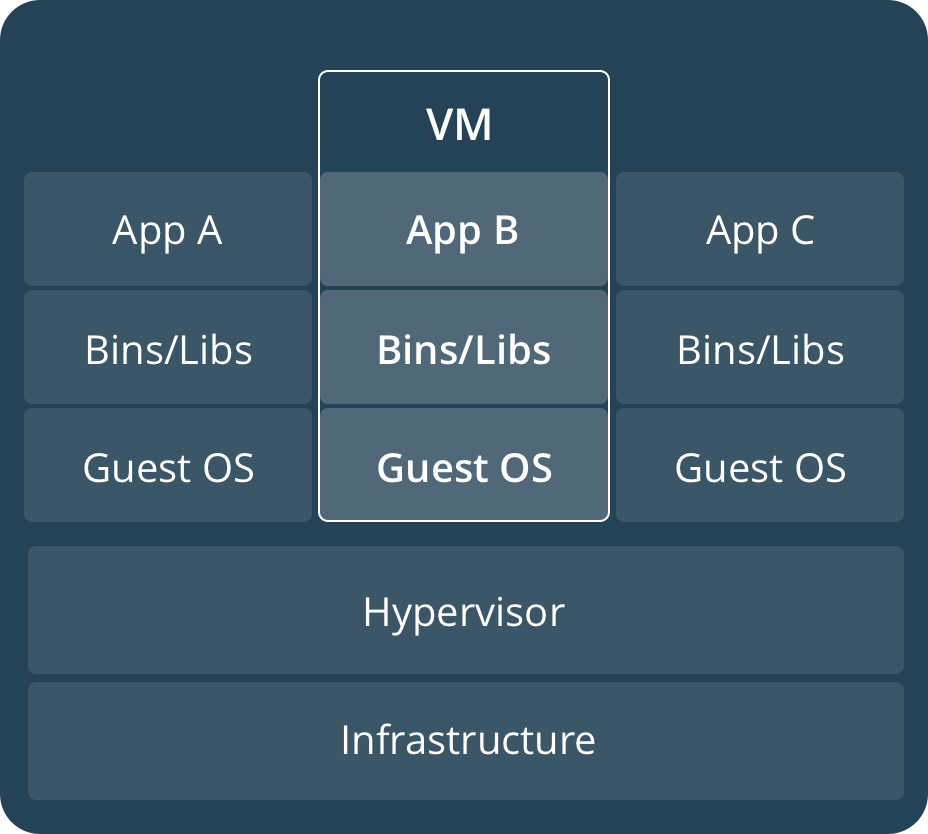
\includegraphics[width=.45\linewidth]{images/vm.png} }}%
	\quad
	\subfloat[Docker container]{{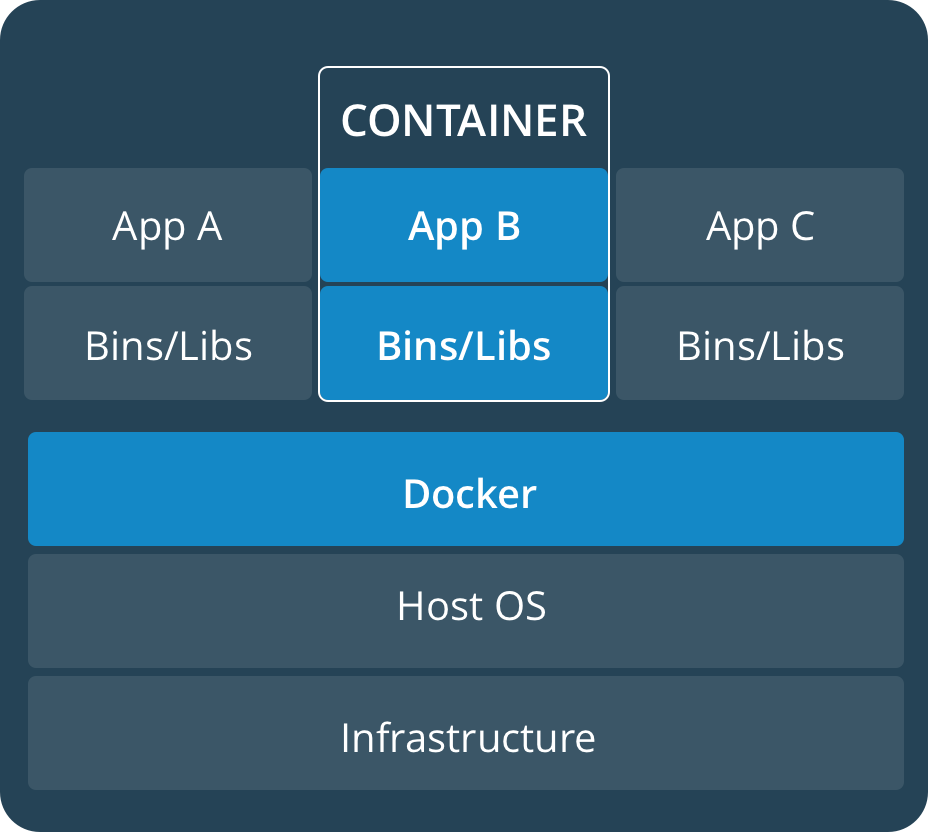
\includegraphics[width=.45\linewidth]{images/dockerContainer.png} }}%
	
	\caption{Comparison between hypervisor-based virtualization and Docker \cite{dockerdocu}}
	\label{fig:docker}
\end{figure}


%A lot of proprietary and custom build environments which VNFs are build for and deployed onto. This limits their effectiveness considerably.
%Virtual Machines, Openstack vs Docker and Kubernetes managing and orchestrating the deployment of network functionality, what are the benefits? What are drawbacks?
\subsection{Cloud-native principles}
What is cloud-native, how do these principles relate to  the networking domain? Whitepapers published by Analysys Mason \cite{evolutionnfv} and Cisco \cite{CNF}
\subsection{CNFs}
Definition, advantages, state-of-the-art, testbed 

% Caveats: Mostly Cisco, lifecycle management, high-performance network, installation and operation

\begin{figure}
	\centering
	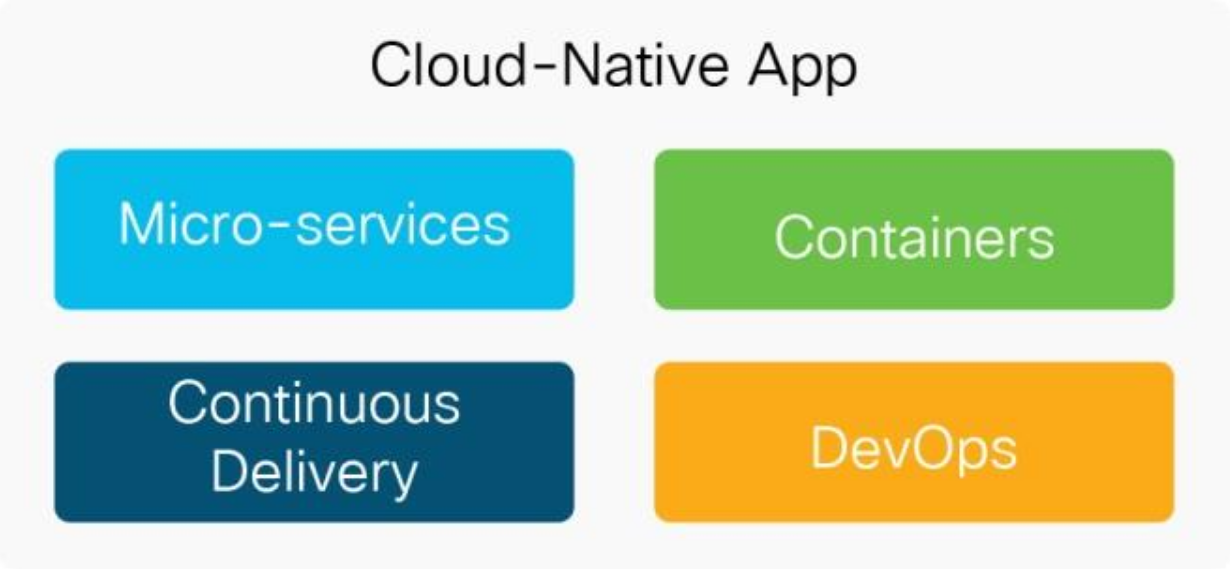
\includegraphics[width=0.75\linewidth]{images/cloudNativeApp.png}
	\caption{The principals of a cloud-native application as defined by the CNF \cite{CNF}}
	\label{img:cloudNativeApp}
\end{figure}

\begin{figure}
	\centering
	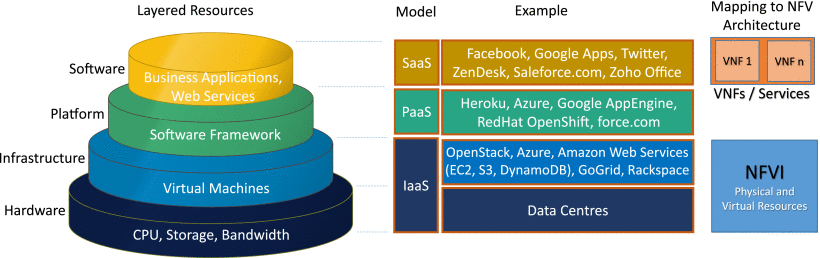
\includegraphics[width=1\linewidth]{images/arch.png}
	\caption{This is the caption \cite{mijumbi2016network}}
	\label{img:arch}
\end{figure}

